\documentclass[12pt,letterpaper]{article}
\usepackage{graphicx,textcomp}
\usepackage{natbib}
\usepackage{setspace}
\usepackage{fullpage}
\usepackage{color}
\usepackage[reqno]{amsmath}
\usepackage{amsthm}
\usepackage{fancyvrb}
\usepackage{amssymb,enumerate}
\usepackage[all]{xy}
\usepackage{endnotes}
\usepackage{lscape}
\newtheorem{com}{Comment}
\usepackage{float}
\usepackage{hyperref}
\newtheorem{lem} {Lemma}
\newtheorem{prop}{Proposition}
\newtheorem{thm}{Theorem}
\newtheorem{defn}{Definition}
\newtheorem{cor}{Corollary}
\newtheorem{obs}{Observation}
\usepackage[compact]{titlesec}
\usepackage{dcolumn}
\usepackage{tikz}
\usetikzlibrary{arrows}
\usepackage{multirow}
\usepackage{xcolor}
\newcolumntype{.}{D{.}{.}{-1}}
\newcolumntype{d}[1]{D{.}{.}{#1}}
\definecolor{light-gray}{gray}{0.65}
\usepackage{url}
\usepackage{listings}
\usepackage{color}

\definecolor{codegreen}{rgb}{0,0.6,0}
\definecolor{codegray}{rgb}{0.5,0.5,0.5}
\definecolor{codepurple}{rgb}{0.58,0,0.82}
\definecolor{backcolour}{rgb}{0.95,0.95,0.92}

\lstdefinestyle{mystyle}{
	backgroundcolor=\color{backcolour},   
	commentstyle=\color{codegreen},
	keywordstyle=\color{magenta},
	numberstyle=\tiny\color{codegray},
	stringstyle=\color{codepurple},
	basicstyle=\footnotesize,
	breakatwhitespace=false,         
	breaklines=true,                 
	captionpos=b,                    
	keepspaces=true,                 
	numbers=left,                    
	numbersep=5pt,                  
	showspaces=false,                
	showstringspaces=false,
	showtabs=false,                  
	tabsize=2
}
\lstset{style=mystyle}
\newcommand{\Sref}[1]{Section~\ref{#1}}
\newtheorem{hyp}{Hypothesis}

\title{Problem Set 3}
\date{Due: November 12, 2026}
\author{Applied Stats/Quant Methods 1}


\begin{document}
	\maketitle
	\section*{Instructions}
	\begin{itemize}
		\item Please show your work! You may lose points by simply writing in the answer. If the problem requires you to execute commands in \texttt{R}, please include the code you used to get your answers. Please also include the \texttt{.R} file that contains your code. If you are not sure if work needs to be shown for a particular problem, please ask.
	\item Your homework should be submitted electronically on GitHub.
	\item This problem set is due before 23:59 on Thursday November 12, 2026. No late assignments will be accepted.

	\end{itemize}

		\vspace{.25cm}
	
\noindent In this problem set, you will run several regressions and create an add variable plot (see the lecture slides) in \texttt{R} using the \texttt{incumbents\_subset.csv} dataset. Include all of your code.\\
	\lstinputlisting[language=R, firstline=37, lastline=37]{PS03_my answers_NF.R} 

	\vspace{.5cm}
\section*{Question 1}
\vspace{.25cm}
\noindent We are interested in knowing how the difference in campaign spending between incumbent and challenger affects the incumbent's vote share. 
	\begin{enumerate}
		\item Run a regression where the outcome variable is \texttt{voteshare} and the explanatory variable is \texttt{difflog}.	
		\vspace{.5cm}\\
		We use the built-in R commands to run the regression:
		
		\lstinputlisting[language=R, firstline=47, lastline=47]{PS03_my answers_NF.R} 
		\vspace{4cm}
		
		
		\item Make a scatterplot of the two variables and add the regression line.
		\vspace{.5cm} \\
		Now we can plot the relationship between both variables:
		
		\lstinputlisting[language=R, firstline=51, lastline=56]{PS03_my answers_NF.R} 
		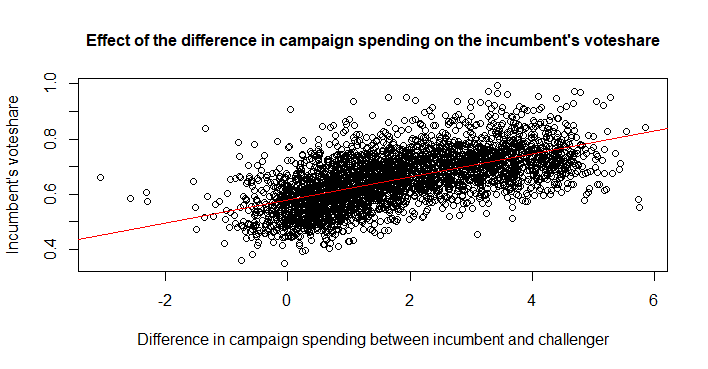
\includegraphics[width=.99\linewidth,height=.5\textheight,keepaspectratio]{plot1}
		\vspace{1cm}
		
		\item Save the residuals of the model in a separate object.
		\vspace{.5cm} \\
		We save the residuals in "residuals\_reg1":
		\lstinputlisting[language=R, firstline=60, lastline=60]{PS03_my answers_NF.R}
		
		\vspace{6cm}
		
		\item Write the prediction equation.
		\vspace{.5cm} \\
		We look at the summary of the regression to write the prediction equation:
		\lstinputlisting[language=R, firstline=65, lastline=65]{PS03_my answers_NF.R}
		\begin{verbatim}
			Call:
			lm(formula = voteshare ~ difflog, data = data)
			
			Residuals:
			Min       1Q   Median       3Q      Max 
			-0.26832 -0.05345 -0.00377  0.04780  0.32749 
			
			Coefficients:
			Estimate Std. Error t value Pr(>|t|)    
			(Intercept) 0.579031   0.002251  257.19   <2e-16 ***
			difflog     0.041666   0.000968   43.04   <2e-16 ***
			---
			Signif. codes:  0 ‘***’ 0.001 ‘**’ 0.01 ‘*’ 0.05 ‘.’ 0.1 ‘ ’ 1
			
			Residual standard error: 0.07867 on 3191 degrees of freedom
			Multiple R-squared:  0.3673,	Adjusted R-squared:  0.3671 
			F-statistic:  1853 on 1 and 3191 DF,  p-value: < 2.2e-16
		\end{verbatim}
		Taking the values from the intercept and difflog, we get this prediction equation: \\
		Y = 0.579031 + X*0.041666          ,or:\\
		Voteshare = 0.579031 + difflog*0.041666\\
		or, rounded: \\
		\textbf{Voteshare = 0.58 + difflog*0.04}	\\
		
		We can make the following interpretations:
		\begin{itemize}
			\item When there is no difference in campaign spending between incumbent and challenger, the expected incumbent's voteshare is 0.58 units.
			\item On average, a one-unit increase in the difference in campaign spending between incumbent and challenger leads to a 0.04 unit increase in the incumbent's voteshare.
		\end{itemize}
		
		
		
	\end{enumerate}
	
\newpage

\section*{Question 2}
\noindent We are interested in knowing how the difference between incumbent and challenger's spending and the vote share of the presidential candidate of the incumbent's party are related.	\vspace{.25cm}
	\begin{enumerate}
		\item Run a regression where the outcome variable is \texttt{presvote} and the explanatory variable is \texttt{difflog}.
		\vspace{.5cm}	\\
		We use the built-in R commands to run the regression:
		
		\lstinputlisting[language=R, firstline=80, lastline=80]{PS03_my answers_NF.R} 
		\vspace{1cm}
		
		
		\item Make a scatterplot of the two variables and add the regression line.
		\vspace{.5cm} \\
		Now we can plot the relationship between both variables:
		
		\lstinputlisting[language=R, firstline=85, lastline=91]{PS03_my answers_NF.R} 
		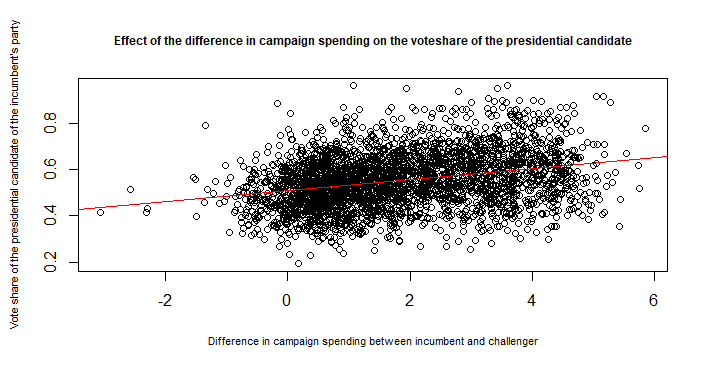
\includegraphics[width=.99\linewidth,height=.5\textheight,keepaspectratio]{plot2}
		\vspace{1cm}
		
		
		\item Save the residuals of the model in a separate object.		\vspace{.5cm} \\
		We save the residuals in "residuals\_reg2":
		\lstinputlisting[language=R, firstline=95, lastline=95]{PS03_my answers_NF.R}
		
		\vspace{.5cm}
		\item Write the prediction equation.
		\vspace{.5cm} \\
		We look at the summary of the regression to write the prediction equation:
		\lstinputlisting[language=R, firstline=99, lastline=99]{PS03_my answers_NF.R}
		\begin{verbatim}
			Call:
			lm(formula = presvote ~ difflog, data = data)
			
			Residuals:
			Min       1Q   Median       3Q      Max 
			-0.32196 -0.07407 -0.00102  0.07151  0.42743 
			
			Coefficients:
			Estimate Std. Error t value Pr(>|t|)    
			(Intercept) 0.507583   0.003161  160.60   <2e-16 ***
			difflog     0.023837   0.001359   17.54   <2e-16 ***
			---
			Signif. codes:  0 ‘***’ 0.001 ‘**’ 0.01 ‘*’ 0.05 ‘.’ 0.1 ‘ ’ 1
			
			Residual standard error: 0.1104 on 3191 degrees of freedom
			Multiple R-squared:  0.08795,	Adjusted R-squared:  0.08767 
			F-statistic: 307.7 on 1 and 3191 DF,  p-value: < 2.2e-16
		\end{verbatim}
		Taking the values from the intercept and difflog, we get this prediction equation: \\
		Y = 0.507583 + X*0.023837          ,or:\\
		presvote = 0.507583 + difflog*0.023837   \\
		or, rounded: \\
		\textbf{Presvote = 0.51 + difflog*0.02}	\\
		
		We can make the following interpretations:
		\begin{itemize}
			\item When there is no difference in campaign spending between incumbent and challenger, the expected vote share of the presidential candidate of the incumbent's party is 0.51 units. \\
			\item On average, a one-unit increase in the difference in campaign spending between incumbent and challenger leads to a 0.02 unit increase in the vote share of the presidential candidate of the incumbent's party.
		
		\end{itemize}
	\end{enumerate}
	
	\newpage
\section*{Question 3}

\noindent We are interested in knowing how the vote share of the presidential candidate of the incumbent's party is associated with the incumbent's electoral success.
	\vspace{.25cm}
	\begin{enumerate}
		\item Run a regression where the outcome variable is \texttt{voteshare} and the explanatory variable is \texttt{presvote}.
		\vspace{.5cm}	
		
		We use the built-in R commands to run the regression:
		
		\lstinputlisting[language=R, firstline=115, lastline=115]{PS03_my answers_NF.R} 
		\vspace{1cm}
		
		
		\item Make a scatterplot of the two variables and add the regression line. 
		\vspace{.5cm} \\
		Now we can plot the relationship between both variables:
		
		\lstinputlisting[language=R, firstline=120, lastline=125]{PS03_my answers_NF.R} 
		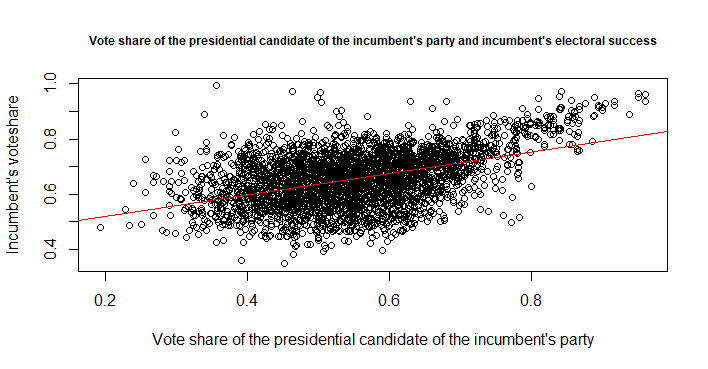
\includegraphics[width=.99\linewidth,height=.5\textheight,keepaspectratio]{plot3}
		\vspace{1cm}
		
			
		\item Write the prediction equation.
		\vspace{.5cm} \\
		We look at the summary of the regression to write the prediction equation:
		\lstinputlisting[language=R, firstline=130, lastline=130]{PS03_my answers_NF.R}
		\begin{verbatim}
			Call:
			lm(formula = voteshare ~ presvote, data = data)
			
			Residuals:
			Min       1Q   Median       3Q      Max 
			-0.27330 -0.05888  0.00394  0.06148  0.41365 
			
			Coefficients:
			Estimate Std. Error t value Pr(>|t|)    
			(Intercept) 0.441330   0.007599   58.08   <2e-16 ***
			presvote    0.388018   0.013493   28.76   <2e-16 ***
			---
			Signif. codes:  0 ‘***’ 0.001 ‘**’ 0.01 ‘*’ 0.05 ‘.’ 0.1 ‘ ’ 1
			
			Residual standard error: 0.08815 on 3191 degrees of freedom
			Multiple R-squared:  0.2058,	Adjusted R-squared:  0.2056 
			F-statistic:   827 on 1 and 3191 DF,  p-value: < 2.2e-16
		\end{verbatim}
		Taking the values from the intercept and presvote, we get this prediction equation: \\
		Y = 0.441330 + X*0.388018          ,or:\\
		Voteshare = 0.441330 + presvote*0.388018\\
		or, rounded: \\
		\textbf{Voteshare = 0.44 + presvote*0.39}	\\
		
		We can make the following interpretations:
		\begin{itemize}
			\item When the vote share of the presidential candidate of the incumbent's party is at 0, the expected incumbent's electoral success is of 0.44 units.
			\item On average, a one-unit increase in the vote share of the presidential candidate of the incumbent's party leads to a 0.39 unit increase in the incumbent's electoral success.
		\end{itemize}	
	\end{enumerate}
	

\newpage	
\section*{Question 4}
\noindent The residuals from part (a) tell us how much of the variation in \texttt{voteshare} is $not$ explained by the difference in spending between incumbent and challenger. The residuals in part (b) tell us how much of the variation in \texttt{presvote} is $not$ explained by the difference in spending between incumbent and challenger in the district.
	\begin{enumerate}
		\item Run a regression where the outcome variable is the residuals from Question 1 and the explanatory variable is the residuals from Question 2.
		\vspace{.5cm}	
		
		We use the built-in R commands to run the regression:
		
		\lstinputlisting[language=R, firstline=151, lastline=151]{PS03_my answers_NF.R} 
		\vspace{1cm}
		
		
		
		\item Make a scatterplot of the two residuals and add the regression line. 
		\vspace{.5cm} \\
		Now we can plot the relationship between both variables:
		
		\lstinputlisting[language=R, firstline=156, lastline=162]{PS03_my answers_NF.R} 
		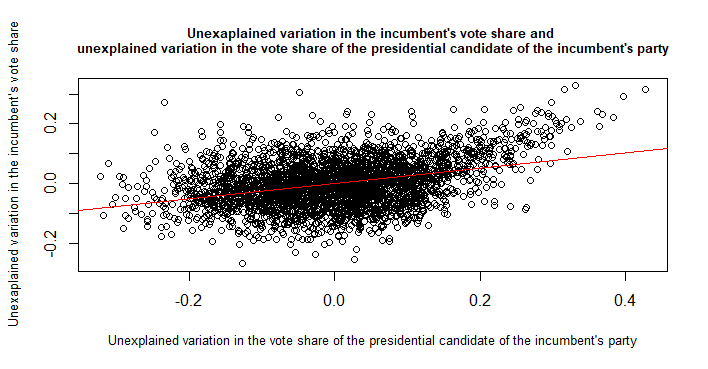
\includegraphics[width=.99\linewidth,height=.5\textheight,keepaspectratio]{plot4}
		\vspace{1cm}
		
		
		\item Write the prediction equation.
		\vspace{.5cm} \\
		We look at the summary of the regression to write the prediction equation:
		\lstinputlisting[language=R, firstline=166, lastline=166]{PS03_my answers_NF.R}
		\begin{verbatim}
			Call:
			lm(formula = residuals_reg1 ~ residuals_reg2, data = data)
			
			Residuals:
			Min       1Q   Median       3Q      Max 
			-0.25928 -0.04737 -0.00121  0.04618  0.33126 
			
			Coefficients:
			Estimate Std. Error t value Pr(>|t|)    
			(Intercept)    -5.934e-18  1.299e-03    0.00        1    
			residuals_reg2  2.569e-01  1.176e-02   21.84   <2e-16 ***
			---
			Signif. codes:  0 ‘***’ 0.001 ‘**’ 0.01 ‘*’ 0.05 ‘.’ 0.1 ‘ ’ 1
			
			Residual standard error: 0.07338 on 3191 degrees of freedom
			Multiple R-squared:   0.13,	Adjusted R-squared:  0.1298 
			F-statistic:   477 on 1 and 3191 DF,  p-value: < 2.2e-16
		\end{verbatim}
		Taking the values from the intercept and the residuals of reg2, we get this prediction equation: \\
		Y = -5.934e-18 + X*2.569e-01          ,or:\\
		Residuals\_reg1 = -5.934e-18 + residuals\_reg2*2.569e-01\\
		or, with the intercept virtually at 0 : \\
		\textbf{Residuals\_reg1 = residuals\_reg2*0.27}	\\
		
	\end{enumerate}
	
	\newpage	

\section*{Question 5}
\noindent What if the incumbent's vote share is affected by both the president's popularity and the difference in spending between incumbent and challenger? 
	\begin{enumerate}
		\item Run a regression where the outcome variable is the incumbent's \texttt{voteshare} and the explanatory variables are \texttt{difflog} and \texttt{presvote}.
		\vspace{.5cm}	
		
		We use the built-in R commands to run the regression:
		
		\lstinputlisting[language=R, firstline=181, lastline=181]{PS03_my answers_NF.R} 
		\vspace{1cm}
		
		
		\item Write the prediction equation.
		\vspace{.5cm} \\
		We look at the summary of the regression to write the prediction equation:
		\lstinputlisting[language=R, firstline=186, lastline=186]{PS03_my answers_NF.R}
		\begin{verbatim}
			Call:
			lm(formula = voteshare ~ difflog + presvote, data = data)
			
			Residuals:
			Min       1Q   Median       3Q      Max 
			-0.25928 -0.04737 -0.00121  0.04618  0.33126 
			
			Coefficients:
			Estimate Std. Error t value Pr(>|t|)    
			(Intercept) 0.4486442  0.0063297   70.88   <2e-16 ***
			difflog     0.0355431  0.0009455   37.59   <2e-16 ***
			presvote    0.2568770  0.0117637   21.84   <2e-16 ***
			---
			Signif. codes:  0 ‘***’ 0.001 ‘**’ 0.01 ‘*’ 0.05 ‘.’ 0.1 ‘ ’ 1
			
			Residual standard error: 0.07339 on 3190 degrees of freedom
			Multiple R-squared:  0.4496,	Adjusted R-squared:  0.4493 
			F-statistic:  1303 on 2 and 3190 DF,  p-value: < 2.2e-16
		\end{verbatim}
		Taking the values from the intercept, difflog and presvote, we get this prediction equation: \\
		Y = 0.4486442 + X1*0.0355431 + X2*0.2568770          , or:\\
		Voteshare = 0.4486442 + difflog*0.0355431 + presvote*0.2568770\\
		or rounded: \\
		\textbf{Voteshare = 0.44 + difflog*0.03 + presvote*0.27}	\\
		\vspace{.5cm} \\
		
		
		\item What is it in this output that is identical to the output in Question 4? Why do you think this is the case?\\
		
		We can see that the residuals of the second regression and the slope coefficient for presvote are the same:\\
		residuals\_reg2 = 2.569e-01 = 0.2569\\
		presvote = 0.2568770
		\vspace{.5cm} \\
		Question 4 allows us to control for the effects of the difflog variable by running a regression of the residuals from our first two models, that is to say the unexplained variation left over.
		\begin{itemize}
			\item In the first model, we found out how much variation of the incumbent’s vote share was explained by the difference in campaign spending between incumbent and challenger.
			\item In the second model, we found out how much variation of the vote share of the presidential candidate of the incumbent's party was explained by the difference between incumbent and challenger's spending.
		\end{itemize}
		With the residuals, we can isolate and calculate the effect of the incumbent presidential candidate's vote share (presvote) on the incumbent’s vote share (voteshare) of the party. \\
		That is why our isolated estimated coefficient for the incumbent presidential candidate's vote share (presvote) is the same as the estimated coefficient for the incumbent presidential candidate's vote share (presvote) \textbf{while controlling for} the difference in campaign spending between incumbent and challenger (difflog).
		
		
	\end{enumerate}




\end{document}
